\documentclass[tikz,border=2pt]{standalone}
\usepackage{pgfplots}
\usepgfplotslibrary{fillbetween}
\pgfplotsset{compat=1.7}

\begin{document}
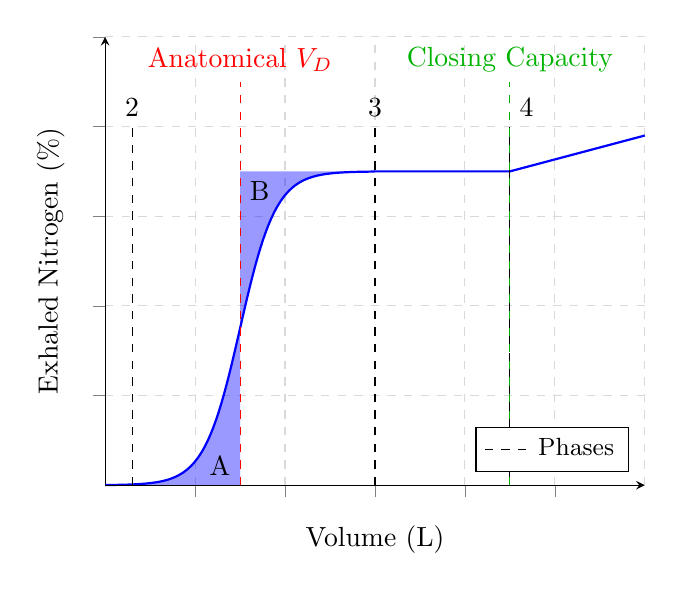
\begin{tikzpicture}

    \begin{axis}[
        axis x line=middle,
        axis y line=middle,
        grid = major,
        grid style={dashed, gray!30},
        xmin=0,     % start the diagram at this x-coordinate
        xmax= 6,    % end   the diagram at this x-coordinate
        ymin= 0,     % start the diagram at this y-coordinate
        ymax= 100,   % end   the diagram at this y-coordinate
        %axis background/.style={fill=white},
    	  x label style={at={(axis description cs:0.5,-0.1)},anchor=north},
	  y label style={at={(axis description cs:-0.1,.5)},rotate=90,anchor=south},
	  xticklabels={},
	 yticklabels={},
	 ylabel near ticks,
	xlabel near ticks,
        xlabel=Volume (L),
        ylabel=Exhaled Nitrogen (\%),
        tick align=outside,
        enlargelimits=false,
clip=false,
legend pos = south east,
legend style={font=\small, cells={align=left}}]

\addlegendentry{Phases}
\addlegendimage{black, thin,dashed};

     \plot[name path=curve1, domain=0:1.5, blue, thick,samples=500] {70*(1/(1+exp(-5*(x-1.5))))};
     \plot[name path=curve2, domain=1.5:3, blue, thick,samples=500] {70*(1/(1+exp(-5*(x-1.5))))};
	\plot[name path=bottom, domain=0:1.5] {0} node[above left]{A} ;	
	\plot[name path=top, domain=1.5:3, draw=none] {70} node[below right, pos=0]{B};	
      \addplot[fill=blue,opacity=0.4] fill between [of=curve1 and bottom];
      \addplot[fill=blue,opacity=0.4] fill between [of=curve2 and top];
	\draw[blue, thick] (axis cs: 3, 70) -- (axis cs: 4.5, 70) -- (axis cs: 6, 78);


	\draw[black, thin, dashed] (axis cs: 0.3,0) -- (axis cs: 0.3, 80) node[above, black]{2};
	\draw[red, thin,dashed] (axis cs: 1.5,0) -- (axis cs: 1.5, 90) node[above, red]{Anatomical $V_D$};
	\draw[black, thin, dashed] (axis cs: 3,0) -- (axis cs: 3, 80) node[above, black]{3};
	\draw[green!70!black, thin,dashed] (axis cs: 4.5,0) -- (axis cs: 4.5, 90) node[above]{Closing Capacity};
	\draw[black, thin, dashed] (axis cs: 4.5,1.82) -- (axis cs: 4.5, 80) node[above right, black]{4};


\end{axis}

\end{tikzpicture} 
\end{document}

